\chapter{Enfoque bayesiano}

En esta sección complementaremos el enfoque visto hasta ahora en cuanto a la incorporación de un modelo para la incertidumbre asociada al parámetro $\theta$. En el paradigma bayesiano, consideraremos que el parámetro es una variable aleatoria, es decir, $\Theta$, la cual para una realización particular tomar el valor $\Theta = \theta$. Esto nos permite información \emph{a priori} sobre la estimación a realizar, lo que permite, en muchos casos, ayudar a la inferencia. Una diferencia conceptual entre ambos enfoques, es que la estadística frecuentista evita la subjetividad, mientras que la estadística bayesiana se basa en la convicción del(a) investigador(a), para emitir juicios sobre una hipótesis.

En este capítulo, se estudiará la estadística bayesiana y se introducirán los mismos conceptos vistos anteriormente desde el punto de vista bayesiano.




\section{Contexto y definiciones principales}

\begin{definition}[Distribución a priori]
La información, sesgos y cualquier otra característica conocida de $\Theta$ codificadas mediante la propia ley de probabilidad de esta VA, la cual tiene densidad $p(\theta)$, nos referimos a esta como la \emph{densidad a priori} o simplemente \emph{prior}.
\end{definition}

Con esta definición, podemos ver que la densidad conjunta de las VAs $X,\Theta$ pueden ser expresadas combinando la densidad a priori con el modelo visto en las secciones anteriores, es decir, 
\begin{equation}
    p(x,\theta) = p(x|\theta)p(\theta)
    \label{eq:joint_bayes}
\end{equation}
donde hemos escrito $p(x|\theta)$ en vez de $p_\theta(x)$ para hacer explícito que ahora consideramos el parámetro como una variable aleatoria. 

Adicionalmente, con la distribución conjunta en la ecuación \eqref{eq:joint_bayes}, podemos definir:

\begin{definition}[Distribución marginal]
La distribución de $X$, obtenida mediante la desintegración de parámetro $\Theta$ del par $(X,\Theta)$, es decir 
\begin{equation}
    p(x) = \int_\Omega p(x|\theta)p(\theta)\d\theta
\end{equation}
es conocida como distribución marginal de $X$.
\end{definition}

Consideremos ahora que tenemos un conjunto de observaciones denotado por $\mathcal{D}$, de un modelo estadístico con parámetro $\Theta$, entonces podemos definir

\begin{definition}[Función de verosimilitud]
La densidad de probabilidad evaluada en un conjunto de observaciones $\cD$ como función del valor del parámetro $\Theta$, es decir 
\begin{align}
    L: \Omega &\rightarrow \R\\
    \theta&\mapsto l(\theta) = L_\cD(\theta) = p(\cD|\theta),
\end{align}
recibe el nombre de función de verosimilitud, o en inglés, \emph{likelihood}. 
\label{función_verosimilitud}
\end{definition}
\begin{remark}
La función de verosimilitud no es una densidad de probabilidad, es decir, no es cierto que
\begin{equation}
    \int_\Omega L(\theta)\d\theta = 1
\end{equation}
\end{remark}

\begin{remark}
Dado que la función función de verosimilitud usualmente adquiere una forma exponencial (como por ejemplo en el caso de la familia exponencial), hay ocasiones en donde es conveniente usar la \emph{log-verosmilitud}, esto es, 
\begin{equation}
l(\theta)=\log L(\theta)=\log p(\cD|\theta).
\end{equation}
Esta formulación será particularmente útil cuando queramos optimizar la verosimilitud. 
\end{remark}

\begin{remark}
En general (pero no siempre) asumimos observaciones $\cD = {X_1,\ldots,X_n}$, $X_i\sim p(x|\theta)$, que son i.i.d. En cuyo caso, la verosimilitud factoriza de la forma $L_\cD(\theta) = \prod_{i=1}^n L_{X_i}(\theta)$, con lo cual la log-verosimilitud toma la forma: 
\begin{equation}
l_\cD(\theta) = \sum_{i=1}^nl_{X_i}(\theta)
\end{equation}
\end{remark}

\begin{example}
Considere los datos $\cD = \{x_1,...,x_n\}$, donde $x_i$ es la observación de una VA $X_i\sim \mathcal{N}(\mu,\sigma^2)$ iid con $\sigma^2$ conocido. La función  de verosimilitud de $\mu$ está dada por:

\begin{align}
L(\mu)=p(\cD|\mu)&=\prod_{i=1}^{n} \frac{1}{\sqrt{2 \pi \sigma^{2}}} 
\exp\left(\frac{-1}{2\sigma^{2}}(x_i-\mu)^{2}\right)\nonumber\\
&= \left(\frac{1}{\sqrt{2 \pi \sigma^{2}}}\right)^{n} \exp\left(\frac{-1}{2 \sigma^{2}} \sum_{i=1}^{n} (x_i - \mu )^{2}\right).
\end{align}

Luego, la log-verosimilitud está dada por:
\begin{equation}
    l(\mu)= \log L(\mu) = -\frac{n}{2} \log(2 \pi \sigma^{2}) + \frac{-1}{2\sigma^{2}} \sum_{i=1}^{n} (x_i - \mu )^{2}.
\end{equation}

\end{example}

Ahora estamos en condiciones de definir el elemento central de la inferencia bayesiana, sobre el cual todo el proceso de inferencia toma lugar. 

\begin{definition}[Distribución posterior]
\label{dist_posterior}
Dado el conjunto de observación $\cD$ la distribución \emph{posterior} del parámetro, es decir, considerando la inforamción reportada por los datos $\cD$, está dada por el teorema de Bayes mediante
\begin{align}
    p(\theta|\cD) = \frac{p(\cD)|\theta)p(\theta)}{p(\cD)}  \propto p(\mathcal{D}|\theta) p(\theta) \label{eq:posterior_def}
\end{align}

donde: 
\begin{itemize}
    \item $p(\theta)$ es el prior del parámetro.
    \item $p(\theta|\mathcal{D})$ es la posterior del parámetro. 
    \item $p(\mathcal{D}|\theta)$ es la verosimilitud
    \item $p(\mathcal{D}) = \int\Omega p(\mathcal{D}|\theta)p(\theta)\d \theta $ es la densidad marginal de los datos 
\end{itemize}
\end{definition}

La \emph{transición} de prior a posterior puede ser interpretada como el proceso de incorporar la evidencia de los datos (a través de la función de verosimilitud) para reducir la incertidumbre con respecto del valor del parámetro $\Theta$. De la ecuación \eqref{eq:posterior_def} podemos ver que este proceso, a veces referido como \emph{actualización bayesiana}, equivale a multiplicar por la verosimilitud, para luego normalizar, garantizando que $p(\theta|\cD)$ es en efecto una densidad de probabilidad. 

\begin{remark}
El símbolo $\propto$ en la ecuación \eqref{eq:posterior_def} es usado para indicar que el lado izquierdo es igual al lado derecho salvo una constante de proporcionalidad que depende de $\mathcal{D}$ y no de $\theta$. Con esto, cuando estemos calculando la posterior, solo nos enfocaremos en \emph{una versión proporcional}, pues luego la densidad posterior se puede encontrar mediante la normalización de esta última.
\end{remark}

\begin{example}[Posterior modelo Bernoulli]
\label{ej_post_bernoulli_1}
Sea $\theta$ la probabilidad de obtener cara al lanzar una moneda, y sean $X_1,..X_n$ $n$ resultados obtenidos al lanzar la moneda. Si no sabemos nada de $\theta$ antes del experimento, hace sentido tomar su prior como una distribución que de igual probabilidad a todo espacio de parámetros, es decir: $\theta \sim Unif(0,1)$. Notemos que el prior encapsula la infromación que tenemos antes del experimento. Modelamos $X_1,..X_n \sim Bernoulli(\theta)$. Entonces: 
$$
p(X_1,..X_n|\theta)=\prod_{i=1}^{n} \theta^{X_i} (1-\theta)^{1-X_i} = 
\theta^{\sum_{i=1}^{n} X_i} (1-\theta)^{n-\sum_{i=1}^{n}X_i}
$$
Notemos que en este caso, podemos calcular la distribución $p(X_1,..,X_n)$:
$$
p(X_1,..,X_n)=\int_{0}^{1} \theta^{\sum_{i=1}^{n} X_i} (1-\theta)^{n-\sum_{i=1}^{n}X_i} d\theta = B\left(\sum_{i=1}^{n} X_i +1 , n- \sum_{i=1}^{n} X_i +1 \right),
$$
donde $B(x,y)$ es la función beta:
$$
B(x,y)=\dfrac{\Gamma(x)\Gamma(y)}{\Gamma(x+y)}.
$$
Sea $s= \sum_{i=1}^{n}X_i$. Entonces la distribución a posteriori será:

$$
p(\theta|X_1,..X_n)= \dfrac{p(X_1,..X_n|\theta)}{p(X_1,..,X_n)} = \dfrac{1}{B(s+1,n-s+1)} \theta^{s} (1-\theta)^{n-s}.
$$

\end{example} 

Usualmente, es experimentos reales, los datos  $x_1,...,x_n$ son recibidos de forma secuencial, es decir, \emph{en línea}. De esta forma, es relevante notar que en primer lugar se observa $x_1$ primero, luego $x_2$, y así sucesivamente. \\

Consecuentemente, si se asume el prior para el parámetro $\theta$ dado por $p(\theta)$, es posible hacer la actualización bayesiana \emph{en línea} (o de forma adaptativa o continual), lo cual implica una corrección del modelo cada vez que se observan más datos. \\
Luego de observar $x_1$, la posterior $p(\theta|x_1)$ puede ser calculada como: 
$$
p(\theta|x_1) \propto p(x_1|\theta) p(\theta).
$$

Luego, al observar $x_2$, usamos el hecho que $X_1$ y $X_2$ son condicionalmente independientes dado $\theta$ y obtenemos: 
$$
p(\theta | x_1,x_2) \propto 
p(x_2|\theta) p(\theta|x_1) \propto p(x_1 |\theta) p(x_2|\theta) p(\theta) . 
$$
Con lo que para el caso general tenemos que 
$$
p(\theta | x_1,..x_n) \propto p(x_n|\theta) p(\theta|x_1,..x_{n-1}) \propto p(\theta) \prod_{i=1}^n p(\theta | x_i).
$$

\begin{remark}
Cuando las observaciones $\cD$ son condicionalmente independientes dado el parámetro $\theta$, entonces, la posterior $p(\theta|\cD)$ factoriza en las verosimilitudes de cada uno de los datos. 
\end{remark}

\begin{remark}
En la actualización bayesiana en línea, la posterior de la etapa $n$ sirve de prior de la etapa $n+1$.
\end{remark}


\section{Priors Conjugados}

La actualización bayesiana puede resultar en una posterior solo conocida de forma proporcional (cuando no es posible calcular la distribución marginal $p(x)$) o bien en una distribución que no pertenece a una familia conocida. Una herramienta que asegurar el cálculo de las distribuciones posteriores (incluyendo la constante de normalización) y que esta adopta una forma conocida es a través del uso de \textbf{priors conjugados}.
\begin{definition}

Sea un modelo con verosimilitud $p(x|\theta)$ y un prior sobre $\theta$ con densidad $p(\theta)$. Decimos que $p(\theta)$ es conjugado con la verosimiltud $p(x|\theta)$ si la posterior 
\begin{equation}
	p(\theta|x) = \frac{p(x|\theta)p(\theta)}{p(x)}
\end{equation}
pertenece a la\textit{misma familia} que el prior $p(\theta)$. Donde pertenecer a la misma familia quiere decir que ambas tienen una densidad de probabilidad definida por la misma forma funcional, e.g., $f_\lambda(\theta)$ pero con distintos valores para el \textit{parámetro} $\lambda$, el cual es un \textit{hiperparámetro} del modelo.
\end{definition}


\begin{example}[continuación de Ejemplo \ref{ej_post_bernoulli_1}]
\label{ej_post_bernoulli_2}
Tarea: Verifique si el Ejemplo \ref{ej_post_bernoulli_1} es en efecto uno de prior conjugado. 
\end{example}

\begin{example}[Distribución Multinomial]
Consideremos una variable aleatoria multinomial $X\sim\mul{n,\theta}$ donde $\theta$ pertenece al simplex 
\begin{equation}
	\label{eq:simplex}
  \{\theta\in[0,1]^k:\theta_1 + \cdots + \theta_k = 1 \}.
 \end{equation} 
 La distribución multinomial genera vectores $X\in\N^k$ cuya $i-$ésima componente modela la cantidad de veces que ocurre el evento $i$ dentro de $k$ eventos en $n$ intentos. Por ejemplo, si lanzamos un dado balanceado 100 veces, el vector que contiene el conteo de veces que obtenemos cada cara puede modelarse como 
 \begin{equation}
  	\theta_\text{dado} \sim \mul{100,\left[\tfrac{1}{6},\tfrac{1}{6},\tfrac{1}{6},\tfrac{1}{6},\tfrac{1}{6},\tfrac{1}{6}\right]}.
  \end{equation} 
Denotando $X=[x_1,\ldots,x_n]$, observemos que una muestra multinomial $X\sim\mul{n,\theta}$ cumple con 
\begin{equation}
	\{x_i\}_{i=1}^k \subset \{0,1,\ldots,n\},\quad  \sum_{i=1}^kx_i = n.
\end{equation}

Finalmente, la distribución Multinomial está dada por 
\begin{equation}
 	\mul{X;n,\theta} = \frac{n!}{x_1!\cdots x_k!} \theta_1^{x_1}\cdots\theta_k^{x_k},
 \end{equation} 
 y es la generalización de las distribuciones: 
\begin{itemize}
	\item Bernoulli cuando $k=2$ y $n=1$; pues $\ber{X;\theta} = \theta^{x} (1-\theta)^{1-x}$
	\item Categórica (o \emph{multinoulli}): cuando $n=1$; pues $\cat{X;\theta} = \theta_1^{x_1}\cdots\theta_k^{x_k}$
	\item Binomial: cuando $k=2$; pues $\bin{X;n,\theta} = \binom{n}{x} \theta^{x}(1-\theta)^{n-x}$
\end{itemize}
\end{example}

Observemos que el parámetro $\theta$ en la distribución multinomial (y las otras tres) es precisamente una distribución de probabilidad (discreta). Es decir, el construir un prior $p(\theta)$ implica definir una distribución sobre distribuciones discretas.  


\begin{definition}[Distribución de Dirichlet]
Consideremos la  distribución de Dirichlet
\begin{equation}
	\theta \sim \dir{\theta|\alpha} = \frac{1}{B(\alpha)} \prod_{i=1}^k \theta_i^{\alpha_i-1},
\end{equation}
donde $\alpha = (\alpha_1,\ldots,\alpha_k)$ es el parámetro de concentración y la constante de normalización está dada por $B(\alpha)=\prod_{i=1}^k\Gamma(\alpha_i)/\Gamma(\sum_{i=1}^k\alpha_i)$. El soporte de esta distribución es el simplex presentado en la ecuación \eqref{eq:simplex}.
\end{definition}


En el caso $k=3$, la distribución de Dirichlet puede ser graficada en el simplex de 2 dimensiones. La Figura \ref{fig:dist_Dirichlet} presenta tres gráficos para distintos valores del parámetro de concentración. 

\begin{figure}[H]

\includegraphics[width=0.3\textwidth]{img/dirichlet111.png}
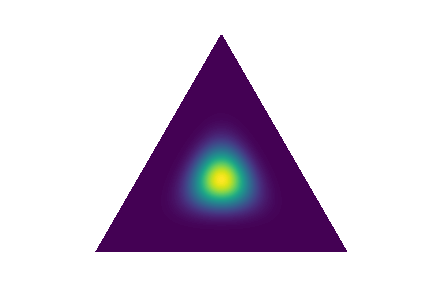
\includegraphics[width=0.3\textwidth]{img/dirichlet101010.png}
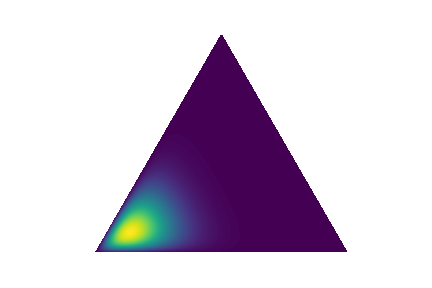
\includegraphics[width=0.3\textwidth]{img/dirichlet1022.png}
\caption{Distribuciones Dirichlet para $k=3$ con parámetros de concentración $\alpha$ (desde izquierda a derecha) dado por $[1,1,1]$, $[10,10,10]$ y $[10,2,2]$. }.
\label{fig:dist_Dirichlet}
\centering
\end{figure}


Veamos a continuación que la distribución de Dirichlet es conjugada al modelo Multinomial, y consecuentemente para Bernoulli, Categórica y Binomial. En efecto, si $\theta \sim \dir{\theta;\alpha}$ y $X\sim\mul{X;n,\theta}$, entonces

\begin{align}
	p(\theta|x) &= \frac{\mul{x;n,\theta}\dir{\theta;\alpha}}{p(x)}\nonumber\\
				&=  \frac{n!}{ x_1!\cdots x_k!p(x) B(\alpha)} \prod_{i=1}^k \theta_i^{x_i + \alpha_i-1}\nonumber\\
				&=  \frac{1}{B(\alpha')} \prod_{i=1}^k \theta_i^{\alpha'_i-1}
				\label{eq:dirichlet_post}
\end{align}
donde $\alpha' = (\alpha'_1,\ldots,\alpha'_k) = (\alpha'_1 + x_1,\ldots,\alpha'_k+ x_k)$ es el nuevo parámetro de concentración.

\begin{example}
	Consideremos $\alpha = [1,2,3,4,5]$ y generemos una muestra de $\theta\sim\dir{\theta|\alpha}$. El siguiente código genera, grafica e imprime esta muestra. 
	\begin{lstlisting}[language=Python]
	import numpy as np
	alpha = np.array([1,2,3,4,5]) 
	theta = np.random.dirichlet(alpha)
	plt.bar(np.arange(5)+1, theta);
	print(f'theta = {theta}')
\end{lstlisting}
En nuestro caso, obtuvimos los parámetros $ \theta = [0.034, 0.171, 0.286, 0.185, 0.324]$.

 Ahora, usaremos un prior Dirichlet sobre $\theta$ con $\alpha_p = [1,1,1,1,1]$ para calcular la posterior de acuerdo a la ecuación \eqref{eq:dirichlet_post}. La Figura \ref{fig:post_Dirichlet} muestra 50 muestras de la distribución posterior para distintas cantidades de observaciones entre 0 y  $ 10^5$. 

\begin{figure}[H]
\centering
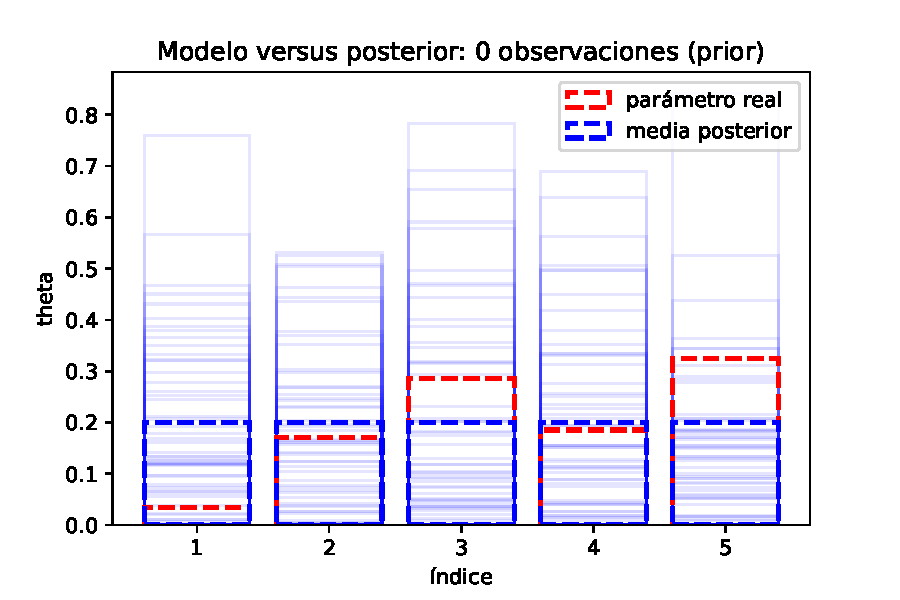
\includegraphics[width=0.3\textwidth]{img/post_dirichlet_0.pdf}
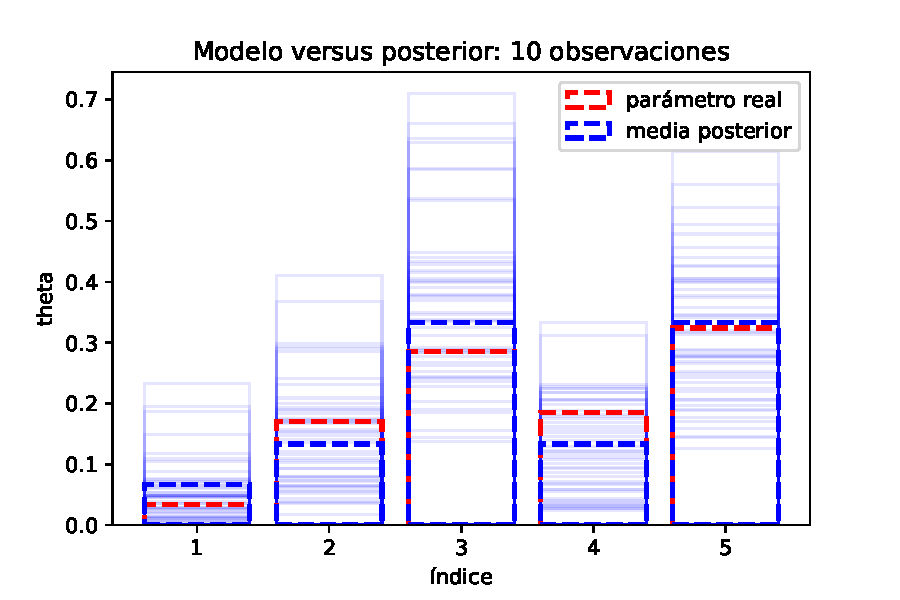
\includegraphics[width=0.3\textwidth]{img/post_dirichlet_10.pdf}
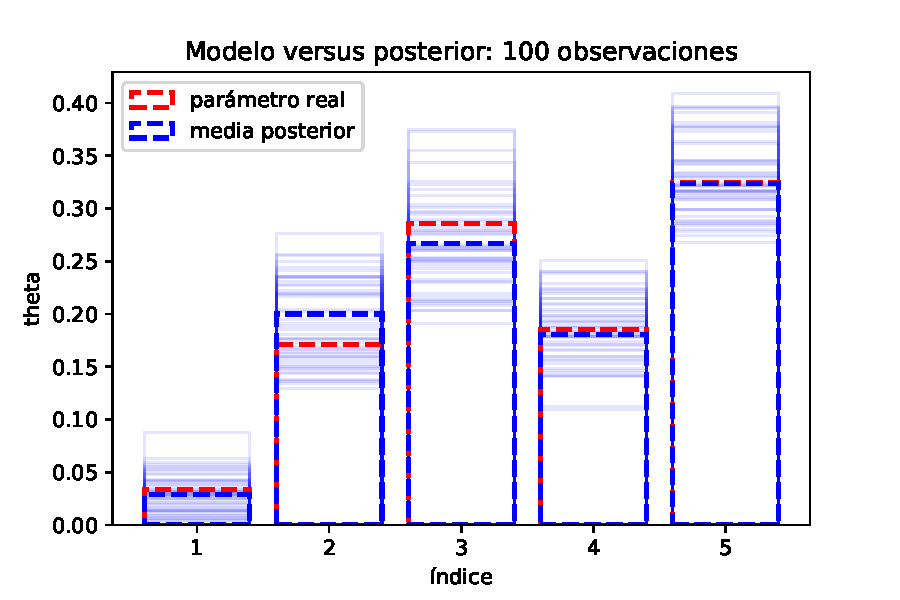
\includegraphics[width=0.3\textwidth]{img/post_dirichlet_100.pdf}\\
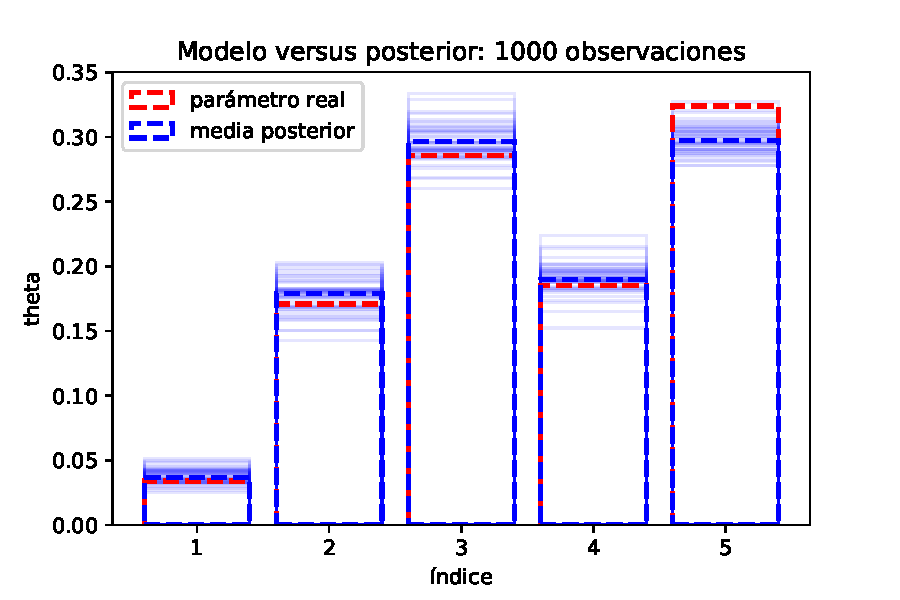
\includegraphics[width=0.3\textwidth]{img/post_dirichlet_1000.pdf}
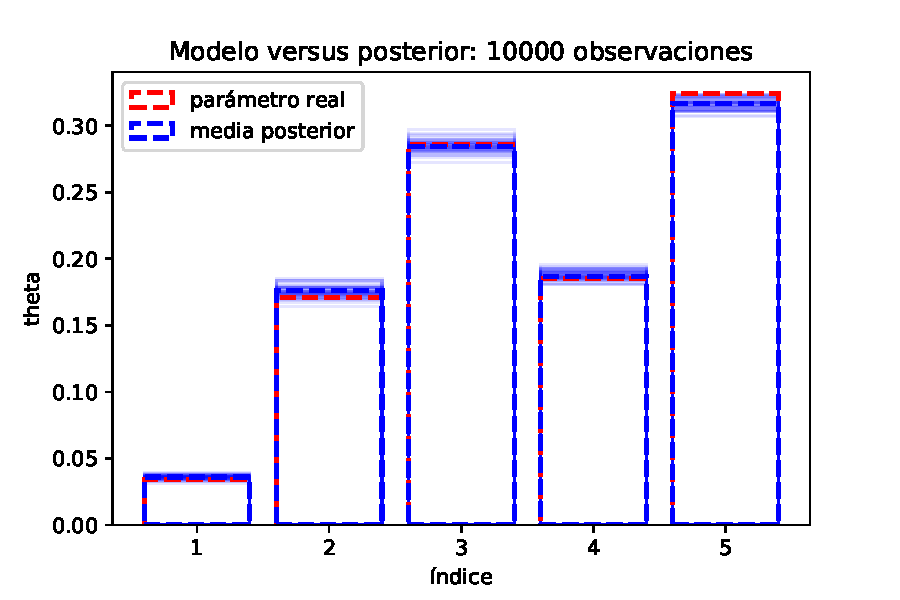
\includegraphics[width=0.3\textwidth]{img/post_dirichlet_10000.pdf}
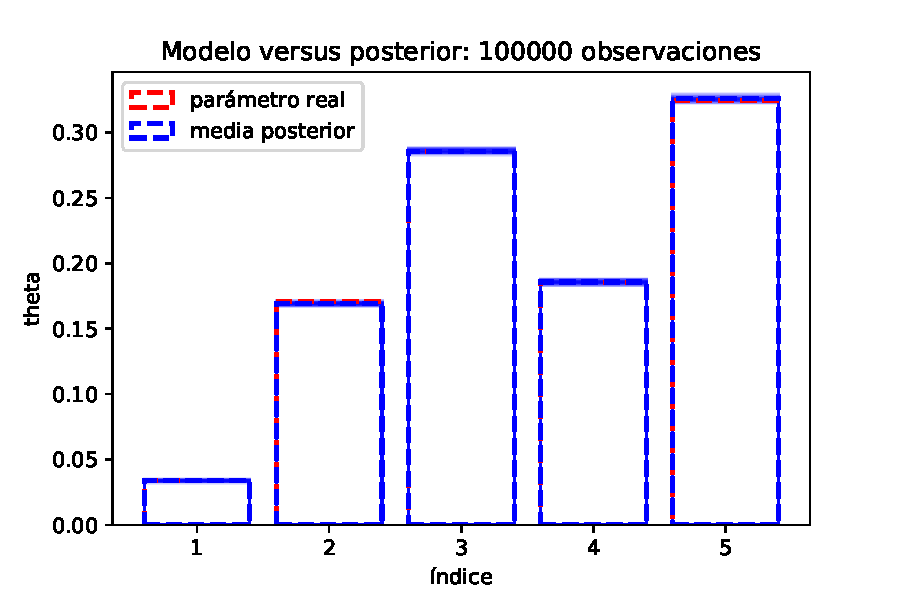
\includegraphics[width=0.3\textwidth]{img/post_dirichlet_100000.pdf}
\caption{Concentración de la distribución posterior en torno al parámetro real para un modelo $X\sim\mul{\theta}$ y una distribución a priori Dirichlet $\theta\sim\dir{\alpha}$. Se considera desde 0 hasta $10^5$ observaciones y cada gráfico (desde izquierda-arriba hasta derecha-abajo) muestra el parámetro real (linea roja quebrada), la media posterior (línea azul quebrada) y 50 muestras de la posterior (azul claro). Observe cómo la distribución a priori (línea azul quebrada en la primera figura) pierde importancia a medida que el número de observaciones aumenta.}
\label{fig:post_Dirichlet}
\end{figure}
\end{example}


\begin{example} \textbf{Modelo gaussiano ($\sigma^2$ conocido).} Consideremos el prior sobre la media $p(\mu) = \cN(\mu_0,\sigma_0^2)$, con lo que la posterior está dada por  
 \begin{align}
 	p(\mu|\mathcal{D}) &\propto \prod_{i=1}^n \frac{1}{\sqrt{2\pi\sigma^2}}\exp\left(-\frac{1}{2\sigma^2}(x_i-\mu)^2\right) \frac{1}{\sqrt{2\pi\sigma_0^2}}\exp\left(-\frac{1}{2\sigma_0^2}(\mu-\mu_0)^2\right)\label{eq:post_normal_mu_1}\\
 	&\propto \exp\left(-\frac{1}{2\sigma^2}\sum_{i=1}^n(x_i-\mu)^2-\frac{1}{2\sigma_0^2}(\mu-\mu_0)^2\right),\label{eq:post_normal_mu_2}
 \end{align} 
 donde la proporcionalidad viene de ignorar la constante $p(\mathcal{D})$ en la primera línea e ignorar todas las contantes que no dependen de $\mu$ en la segunda línea. Recordemos que estas constantes para $\mu$ incluyen a la varianza de $x$, $\sigma^2$, por lo que ignorar esta cantidad es solo posible debido a que estamos considerando el caso en que $\sigma^2$ es conocido. Completando la forma cuadrática para $\mu$ dentro de la exponencial en la ec.~\eqref{eq:post_normal_mu_2}, obtenemos
 \begin{equation}
 	p(\mu|\mathcal{D}) \propto \exp\left(-\frac{1}{2\sigma_n^2}(\mu - \mu_n)^2\right),\label{eq:post_normal_mu_3}
 \end{equation} 
 donde (ya definiremos $\mu_n$ y $\sigma_n^2$ en breve) como $p(\mu|\mathcal{D})$ debe integrar uno, la única densidad de probabilidad proporcional al lado derecho de la ecuación anterior es la Gaussiana de media $\mu_n$ y varianza $\sigma_n^2$. Es decir, la constante de proporcionalidad necesaria para la igualdad en la expresión anterior es
 \begin{equation}
     \int_\R\exp\left(-\frac{1}{2\sigma_n^2}(\mu - \mu_n)^2\right)\d\mu = (2\pi\sigma_n^2)^{n/2}.
 \end{equation} Consecuentemente, confirmamos que el prior elegido era efectivamente conjugado con la verosimilitud gaussiana, con lo que la posterior está dada por la siguiente densidad (gaussiana):
  \begin{equation}
 	p(\mu|\mathcal{D}) = \cN(\mu;\mu_n,\sigma_n^2) = \frac{1}{(2\pi\sigma_n^2)^{N/2}}\exp\left(-\frac{1}{2\sigma_n^2}(\mu - \mu_n)^2\right),\label{eq:post_normal_mu_4}
 \end{equation} 
 donde la media y la varianza están dadas respectivamente  por 
 \begin{align}
 	\mu_n &= \frac{1}{\tfrac{1}{\sigma_0^2} + \tfrac{n}{\sigma^2}} \left(\frac{1}{\sigma_0^2}\mu_0 + \frac{n}{\sigma^2}\bar{x} \right), \quad \text{donde } \bar{x} = \frac{1}{n}\sum_{i=1}^n x_i\label{eq:post_Gm}\\
 	\sigma_n &= \left(\frac{1}{\sigma_0^2} + \frac{n}{\sigma^2}\right)^{-1}.\label{eq:post_Gv}
 \end{align}
\end{example}
\begin{remark}
	La actualización bayesiana transforma los parámetros del prior de  $\mu$ desde  $\mu_0$ y $\sigma_0^2$ hacia $\mu_n$ y $\sigma_n^2$ en las ecs.~\eqref{eq:post_Gm} y \eqref{eq:post_Gv} respectivamente. Notemos que los  parámetros de la posterior son combinaciones (interpretables por lo demás) entre los parámetros del prior y los datos, en efecto, la $\mu_n$ es el promedio ponderado entre  $\mu_0$ (que es nuestro candidato para $\mu$ antes de ver datos) con factor $\sigma_0^{-2}$ y el promedio de los datos $\bar{x}$ con factor $(\sigma^{2}/n)^{-1}$, que a su vez es el estimador de máxima verosimilitud. Es importante también notar que  estos  factores son las varianzas inversas---i.e., precisión---de $\mu_0$ y de $\bar{x}$. Finalmente, observemos que $\sigma_n$ es la \emph{suma paralela} de las varianzas, pues  si expresamos la ec.~\eqref{eq:post_Gv} en términos de \emph{precisiones}, vemos que la precisión inicial $\sigma_0^2$ aumenta un término $\sigma^2$ con cada dato que vemos; lo cual tiene sentido pues con más información es la precisión la que debe aumentar y no la incertidumbre (en este caso representada por la varianza).
\end{remark}
\begin{example} \textbf{Modelo gaussiano ($\mu$ conocido).} Ahora procedemos con el siguiente prior para la varianza, llamado Gamma-inverso:
 \begin{equation}
 	p(\sigma^2)= \text{inv-}\Gamma(\sigma^2;\alpha,\beta) = \frac{\beta^\alpha}{\Gamma(\alpha) (\sigma^2)^{\alpha+1}}\exp(-\beta/\sigma^2)
 \end{equation}
 esta densidad recibe dicho nombre pues es equivalente a modelar la precisión, definida como el recíproco de la varianza $1/\sigma^2$, mediante la distribución Gamma. Los hiperparámetros $\alpha$ y $\beta$ son conocidos como parámetros de forma y de tasa (o precisión) respectivamente. 

 Con este prior, la posterior de la varianza toma la forma:
 \begin{align}
 	p(\sigma^2|\mathcal{D}) &\propto \prod_{i=1}^N \frac{1}{\sqrt{2\pi\sigma^2}}\exp\left(-\frac{1}{2\sigma^2}(x_i-\mu)^2\right) \frac{\beta^\alpha}{\Gamma(\alpha) (\sigma^2)^{\alpha+1}}\exp(-\beta/\sigma^2)\\
 	&\propto  \frac{1}{(\sigma^2)^{N/2+\alpha+1}}\exp\left(-\frac{1}{\sigma^2}\left(\frac{1}{2}\sum_{i=1}^N(x_i-\mu)^2 +\beta\right) \right)\nonumber
 \end{align} 
 donde nuevamente la proporcionalidad ha sido mantenida debido a la remoción de las constantes. Esta última expresión es proporcional a una distribución Gamma inversa con hiperparámetros $\alpha$ y $\beta$ ajustados en base a los datos observados. 


\end{example}




Hay ocasiones en las que el conocimiento a priori sobre el parámetro no puede ser convenientemente expresado mediante una densidad de probabilidad pero sí una densidad que no necesariamente integra uno o incluso es (Lebesgue) integrable. Para reflejar esta idea, se usan priors impropios.

\begin{definition}[Prior impropia] Una distribución a priori impropia es una distribución que no es necesariamente de probabilidad (i.e., no integra 1), pero que de todas formas puede ser utilizada como distribución a priori en el contexto de inferencia bayesiana, pues la distribución posterior correspondiente si es una distribución de probabilidad apropiada. 
\end{definition}

\begin{remark} No es necesario usar la constante de normalización en las densidades a priori Gaussianas (o ninguna otra en realidad).
\end{remark}

\begin{remark} Veamos que un prior impropio puede incluso tener integral infinita, en el caso de la distribución normal $X\sim\cN(X;\mu,1)$,  $\mu\in\R$, podemos elegir $p(\mu)\propto1$ y escribir 
\begin{equation}
	p(\mu|x)\propto p(x|\mu)\cdot 1 = \cN(x;\mu,1) = \cN(\mu;x,1). 
\end{equation}
	
\end{remark}

Considerar distribuciones uniformes impropias como priors no informativas parece tener sentido, pues intuitivamente no estamos dando preferencia (mayor probabilidad a priori) a ningún valor del parámetro por sobre otro. Sin embargo, este procedimiento sufre de una desventaja conceptual.




\section{Estimación y predicción}

\subsection{Estimadores bayesianos}

Si bien ya hemos estudiado el rol del prior en la inferencia bayesiana, hasta ahora no lo hemos considerado en la construcción de estimadores. En particular, el EMV no incorpora conocimiento a priori del parámetro. Con el objetivo de incorporar este conocimiento a priori en el cálculo de estimadores puntales, consideramos que en el caso general, podemos considerar otros estimadores puntuales a través de una función de pérdida asociada a estimar el parámetro $\theta$ mediante el estimador $\hat\theta$ dada por $L(\theta,\hat\theta)$. Con esto podemos definir los conceptos de riesgo y estimador bayesiano.

\begin{definition}[Riesgo bayesiano]
Para una función de pérdida $L(\theta,\hat\theta)$ y un conjunto de observaciones $\cD$, el riesgo bayesiano es la esperanza posterior de dicha función de pérdida, es decir
\begin{equation}
    R(\hat\theta) = \int_\Omega L(\theta,\hat\theta)p(\theta|\cD)\d\theta.
\end{equation}
\end{definition}



\begin{definition}[Estimador bayesiano]
Dado un conjunto de datos $\cD$ y un riesgo bayesiano $R(\theta)$, un estimador bayesiano es uno que minimiza el riesgo bayesiano:
\begin{equation}
    \theta_\text{Bayes}(\cD) = \arg\min_{\Omega} R(\theta).
\end{equation}
donde es implícito que $R(\cdot)$ se define con $\cD$.
\end{definition}

A continuación, se definirán estimadores bayesianos  con distintas funciones de costo o de riesgo.


\begin{definition}[Bayes' Least-Squares (BLS)]
El  caso estándar es la función de pérdida cuadrática $L_2(\theta,\hat\theta) = (\theta-\hat\theta)^2$ la cual resulta en el estimador dado por la media posterior $\theta_\text{Bayes}(\cD) = \E{\theta|\cD}$
\end{definition}


\begin{definition}[Minimum absolute-error (MAE)]

De forma similar,la función de costo $L_1(\theta,\hat\theta) = |\theta-\hat\theta|_1$ resulta en el estimador dado por la mediana posterior.
\end{definition}

Encontrar una función de pérdida para el máximo a posteriori es menos directo. Consideremos en primer lugar el caso $\theta\in\Omega$ discreto y la pérdida ``0-1''
\[   
L_\text{0-1}(\theta,\hat\theta) = 
     \begin{cases}
       0 &\quad\text{si } \theta = \hat\theta,\\
       1 &\quad\text{si no}. 
     \end{cases}
\]

El riesgo de Bayes asociado a $L_\text{0-1}(\theta,\hat\theta)$ (en el caso discreto) toma la forma
\begin{equation}
    R(\hat\theta) = \Prob{\theta\neq\hat\theta|\cD} = 1-\Prob{\theta = \hat\theta|\cD},
\end{equation}
lo cual es minimizado eligiendo $\hat\theta$ tal que $\Prob{\theta = \hat\theta|\cD}$ es máximo, es decir, el MAP. ¿por qué no es posible proceder de esta forma para el caso continuo? ¿cuál es la función de costo asociada al MAP en el caso continuo?

\begin{definition}[Estimador máximo a posteriori]
Sea $\theta \in \Theta$ un parámetro con distribución a posteriori $p(\theta |D)$ definida en todo $\Theta$. Entonces nos referiremos a su estimación puntual dada por: 
$$
\theta_{MAP}= \underset{\Theta}{\arg\max}\ p(\theta|D),
$$

como el estimador \emph{máximo a posteriori} (MAP). Se utiliza la siguiente función de costo:

\[C(a,b)=\begin{cases}
  1, &|a-b|>0\\
  0, \sim
\end{cases}\]
\end{definition}

\begin{remark}
Es posible encontrar el MAP solo teniendo acceso a una versión \emph{proporcional} a la distribución posterior, un escenario usual en inferencia bayesiana, o también mediante la maximización del logaritmo de ésta última. En efecto, 
$$
\theta_{MAP} = \underset{\theta \in \Theta}{\arg\max }\ p(\theta|\mathcal{D}) = \underset{\theta \in \Theta}{\arg\max }\ p(\mathcal{D}|\theta)p(\theta)= \underset{\theta \in \Theta}{\arg\max}\left(\underbrace{\log p(\mathcal{D}|\theta)}_{l(\theta)} + \log p(\theta)\right),
$$
donde hemos encontrado la maximización de  la función de log-verosimilitud, pero ahora junto al log-prior.
\end{remark}

\begin{remark}
Es relevante notar que el estimador MAP es una \emph{modificación} del EMV, pues ambos comparten una parte de la misma función objetivo (verosimilitud) con la diferencia que el MAP además incluye el término \emph{log-prior}. Esto puede entenderse como una regularización de la solución del problema de MV, en donde el término adicional puede representar las propiedades del estimador más allá de que las pueden ser exclusivamente revelada por los datos. 
\end{remark}

\begin{example}[Máximo a posterior para el modelo gaussiano]
En particular, para el modelo lineal y gaussiano que hemos considerado hasta ahora, podemos calcular $\theta_{MAP}$ para un prior Gaussiano de media cero y varianza $\sigma_\theta^2$. Éste está dado por (asumimos la varianza del ruido $\sigma_\epsilon^2$ conocida):	
\begin{align}
	\theta_\text{MAP}^\star 	&= \text{argmax } p(Y|\theta,X)p(\theta)\nonumber\\
	\text{[ind., def.]}\ &= \text{argmax } \prod_{i=1}^N \cN(y_i;\theta^\top x_i,\sigma_\epsilon^2)\cN(\theta;0,\sigma_\theta^2) \nonumber\\
	&= \text{argmax } \prod_{i=1}^N \frac{1}{\sqrt{2\pi}\sigma_\epsilon} \exp\left({\frac{-1}{2\sigma_\epsilon^2}(y_i-\theta^\top x_i)^2}\right)											\frac{1}{(\sqrt{2\pi}\sigma_\theta)^{M+1}} \exp\left({\frac{-||\theta||^2}{2\sigma_\theta^2}}\right) \nonumber\\
	 &= \text{argmax } \frac{1}{\sqrt{2\pi}\sigma_\epsilon} \frac{1}{(\sqrt{2\pi}\sigma_\theta)^{M+1}} \exp\left( \sum_{i=1}^N{\frac{-1}{2\sigma_\epsilon^2}(y_i-\theta^\top x_i)^2} -{\frac{||\theta||^2}{2\sigma_\theta^2}}\right) \nonumber\\
	\text{[log.]}\  &= \text{argmin } \sum_{i=1}^N{(y_i-\theta^\top x_i)^2} +{\frac{\sigma_\epsilon^2}{\sigma_\theta^2}||\theta |^2}.\nonumber 
	\label{eq:MAP_reg_lin}
\end{align}
Podemos ver que eligiendo un prior uniforme o de normal de varianza muy amplia, el MAP es equivalente al EMV. ¿qué significa esto? ¿qué comportamiento differente de EMV promueve el MAP en este caso?
\end{example}






\subsection{Posterior predictiva}

En la inferencia bayesiana las predicciones ocupan un rol relevante, pues luego de realizar inferencia sobre un modelo estadístico, en general estamos interesados estudiar cómo serán los siguientes datos genearados por el modelo. Para esto definiremos la predicción bayesiana de la forma

\begin{definition}[Posterior predictiva]
Para un conjunto de datos $\cD$ y un parámetro $\theta$, la densidad posterior predictiva está dada por
\begin{equation}
    p(x|\cD) = \int_\Omega p(x|\theta)p(\theta|\cD)\d\theta = \E{p(x|\theta) |\cD},
\end{equation}
es decir, el valor esperado del modelo estadístico con respecto a la ley posterior del parámetro (modelo).
\end{definition}
Podemos ahora considerar la posterior predictiva como nuestro modelo \emph{aprendido} y generar datos de él, donde nos encontramos frente al mismo dilema de un estimador puntual como en el caso anterior: es posible considerar muestras aleatorias, la media, la mediana o algún intervalo. 

\begin{remark}
La posterior predictiva es distinta (en general) a la predicción \emph{plug-in}, en donde consideramos en modelo estadístico $p_{\hat\theta}$ en base a un estimador (puntual) cualquiera $\hat\theta$. Desde esa perspectiva, la posterior predictiva equivale a considerar estimadores y modelos puntuales pero integrar todos ellos con respecto a la ley posterior. 
\end{remark}

\newpage


\section{El prior de Jeffreys}

Consideremos $X\sim p(x|\theta)$, $\theta \in [a,b]$, en donde elegimos el prior \textit{no informativo} uniforme dado por 
$$
	p(\theta) =\uni{a,b} = \frac{1}{b-a}.
$$
Consideremos ahora un modelo \textit{reparametrizado} $\eta = e^\theta\in[c,d]$, donde el modelo es expresado como $X\sim q(x|\eta) = p(x|\theta) $. El prior uniforme para el nuevo parámetro es
\begin{equation}
	p(\eta) =\uni{c,d} = \frac{1}{d-c}.
\end{equation}
Observemos que la elección uniforme del parámetro $\theta$ en el intervalo $[a,b]$ es equivalente a elegir $\eta$ según
\begin{equation}
	\tilde{p}(\eta) = p(\theta) \left|\frac{d\theta}{d\eta}\right| = \frac{1}{b-a}\left|\frac{d\log\eta}{d\eta}\right|= \frac{1}{\eta (b-a)},
\end{equation}
es decir, la distribución sobre $\eta$ inducida por $p(\theta)$. Esta distribución por supuesto no es equivalente a elegir $\eta$ uniformemente en el intervalo $[c,d]$. 

\begin{remark}
¿Es un prior uniforme realmente no informativo si luego de elegir otra parametrización este ya no es uniforme? ¿Es posible construir un prior no informativo?
\end{remark}

Una forma de construir un prior que es invariante ante reparametrizaciones es mediante la metodología propuesta por  Harold Jeffreys (1946), el que sugiere elegir un prior proporcional a la raíz cuadrada del determinante de la información de Fisher, es decir,  
\begin{equation}
	p(\theta) \propto \left( I(\theta)\right)^{1/2},
\end{equation}
donde recordemos que la información de Fisher está dada por 
\begin{equation}
	I(\theta) = -\Et{\frac{\partial^2}{\partial\theta^2}\log p(X|\theta)} = \Et{\left(\frac{\partial}{\partial\theta}\log p(X|\theta)\right)^2}.
\end{equation}
Además, si $X_1,\ldots,X_n$ son iid, entonces $I(\theta) = n I_1(\theta)$ y el prior de Jeffreys puede ser expresado como 
\begin{equation}
	p(\theta) \propto  I_1(\theta)^{1/2}.
\end{equation}
Observemos que si $\int_\Omega\sqrt{I(\theta)}\d\theta$ es finito, entonces la constante de proporcionalidad es precisamente esta cantidad. Sin embargo, si esta cantidad es infinita el prior de Jeffreys aún es un prior válido pero impropio, siempre y cuando las posteriores respectivas sí sean propias. 

Veamos ahora que el prior de Jeffreys es invariante bajo reparametrizaciones. Consideremos los modelos relacionados mediante reparametrización dados por 
\begin{equation}
	X\sim p(x|\theta),\ \theta\in\Omega\quad \& \quad X\sim q(x|\eta),\ \eta\in\Gamma,
\end{equation}
donde $\eta = h(\theta)$. Las informaciones de Fisher para ambos modelos, denotadas respectivamente $I_p(\theta)$ e $I_q(\theta)$, están relacionadas mediante
\begin{align}
	I_p(\theta) &= \int_\cX\left(\frac{\partial}{\partial\theta}\log p(x|\theta)\right)^2p(x|\theta)\d x\nonumber\\
				&= \int_\cX\left(\frac{\partial}{\partial\theta}\log q(x|h(\theta))\right)^2q(x|h(\theta))\d x\nonumber\\
				&= \int_\cX\left(\frac{\partial}{\partial\eta}\log q(x|\eta) h'(\theta)\right)^2q(x|\eta)\d x\nonumber\\
				&= \left(h'(\theta)\right)^2 I_q(\eta).
\end{align} 

Observemos ahora que el prior en $\theta$, $p(\theta)$, inducido por el prior de Jeffreys en $\eta$, $p_J(\eta)$, es efectivamente el prior de Jeffreys en $\theta$, $p_J(\theta)$. En efecto, debido al cambio de variable tenemos

\begin{equation}
	p(\theta) = p_J(\eta) \left|\frac{d \eta}{d \theta}\right| = \sqrt{I_q(\eta)}\left|h'(\theta)\right| = \sqrt{I_p(\theta)} = p_J(\theta).
\end{equation}

Como ya mencionamos, la construcción del Prior de Jeffreys surge con la idea de usar un prior que sea invariante bajo transformaciones monótonas y que sea no informativo. ¿Pero cómo se logra esto últmo? Resulta ser que el prior de Jeffreys es el prior uniforme sobre el espacio de parámetros $\Theta$, pero no con la métrica euclidiana. Intuitivamente, la topología que se debe considerar es aquella que calcula la distancia entre dos parámetros $\theta_1$ y $\theta_2$ como la divergencia de Kulback-Liebler entre sus distribuciones asociadas $f(x|\theta_1)$ y $f(x|\theta_2)$.

\section{Intervalos de Credibilidad}

En el concepto (frecuentista) de intervalo de confianza, la  \emph{aleatoriedad} ocurre antes que veamos los datos, pues recordemos que los supuestos de este paradigmas son que el parámetro es fijo y desconocido, y la generación de datos es aleatoria. Con esto, el hecho de encontrar un intervalo de confianza del, e.g., 95\% quiere decir que existe un 95\% de probabilidad de que un intervalo de confianza observado en el futuro (en realidad lo observado son los datos y el intervalo es función de éstos) contengan al parámetro. Esto es contraintuitivo, pues nos gustaría que la {aleatoriedad} ocurriera \emph{después de observar los datos}, es decir, dado los datos $x$ cual es la probabilidad de que el parámetro está dentro de un intervalo dado?

El paradigma bayesiano permite enunciar lo anterior y propone una noción de intervalos de confianza más natural que el enfoque frecuentista, pues para $ C_x\subset \Omega$, la expresión $\mathbb{P}(\theta \in)$ tiene un significado, incluso condicional a $x$. En este caso, le llamamos intervalos de credibilidad a los intervalos de confianza bayesianos. Para diferenciar estos intervalos con el caso frecuentista, veamos la siguiente definición. 

\begin{definition}
Sea $\pi$ el prior del parámetro $\theta$, un conjunto $C_x$ se dice  $\alpha$-creíble si la posterior correspondiente al prior $\pi$ cumple con 
$$
\mathbb{P}(\theta \in C_x |x) = \int_{C_x}p(\theta |x) = 1- \alpha.
$$
\end{definition}

Notemos que al igual que para el caso frecuentista, esta región no está únicamente determinada, pues puede ser centrada, no convexa, concentrada el en origen, etc. Para esto, podemos considerar los siguientes criterios: 

\begin{itemize}
    \item Elegir el intervalo más pequeño, es decir,  el que minimiza el volumen de las regiones $\alpha$-creíbles. Esto motiva la siguiente definición.
    \begin{definition}
    Una región de Alta Densidad Posterior (HPD por su sigla en inglés) denotada mediante 
    $$
    C_{\alpha}  = \left \{ \theta: p(\theta|x) \geq  k_{\alpha}\right \} ,
    $$
    donde $k_{\alpha}$ es la cota más grande tal que: 
    $$
    \mathbb{P}(\theta \in C_{\alpha}|x) = 1- \alpha.
    $$
    \end{definition}

     Observe que para las distribución unimodales, la moda (el máximo a posteriori) estará incluido en este intervalo. 
     
     \item Elegir un intervalo tal que la probabilidad de estar a la izquierda es igual a la probabilidad de esta a la derecha. Este intervalo incluye a la mediana y es llamado \textbf{intervalo de igual colas}
     \item Asumir que la media existe y elegir el intervalo centrado en ésta.
\end{itemize}



\begin{example}
Considere el prior $\theta \sim \pi(\theta) =  \mathcal{N}(0,\tau^{2})$ y una verosimilitud tal que la posterior de $\theta$ es una normal $\mathcal{N}(\mu(x),\omega^{-2})$, con $\omega^{-2}= \tau^{-2} + \sigma^{-2} $
y $\mu(x)=\dfrac{\tau^{2}x}{\tau^2 + \sigma^2}$. Luego: 
$$
C_{\alpha} =[\mu(x) - k_{\alpha}\omega^{-1},\mu(x)+k_{\alpha}\omega^{-1} ],
$$
con $k_{\alpha}$ el $\alpha /2 $-intil de $\mathcal{N}(0,1)$. En particular, si $\tau \to \infty$, $\pi(\theta)$ converge a la medida de Lebesgue en $\R $ y: 
$$
C_{\alpha}= [x - k_{\alpha}\sigma ,x + k_{\alpha}\sigma],
$$
que corresponde al intervalo de confianza clásico para una normal. 
\end{example}


\begin{remark}
    Si los intervalos de confianza y credibilidad para a la media de la gaussiana son el mismo, ¿cuál es la diferencia? 
\end{remark}

\begin{example} Encuentre el 85\%-intervalo creíble de $\lambda$ en $x_1,\ldots, x_n\sim \expo{\lambda}$ cuando el prior es uniforme. Tenemos 
\begin{equation}
    p(\lambda|x_1,\ldots, x_n) \propto \lambda^ne^{-\lambda\sum_i x_i},
\end{equation}
con lo que concluimos que
\begin{equation}
p(\lambda|x_1,\ldots, x_n) = \Gamma(n+1,\sum_i x_i).
\end{equation}

Debemos ahora encontrar $a,b$ tal que 
\begin{equation}
    \int_a^b \frac{(\sum_i x_i)^{n+1}}{\Gamma(n+1)}\lambda^ne^{-\lambda\sum_i x_i}\d\lambda = 0.85
\end{equation}
donde tenemos las 3 opciones mencionadas arriba.
\end{example}

\begin{exercise} Encuentre el intervalo creíble para $\theta$ en el Ejemplo \ref{eq:unif_int_conf}
\end{exercise}





\section{Test de Hipótesis Bayesiano}
 Hasta ahora sólo hemos visto los distintos test de hipótesis desde una perspectiva frecuentista. En todos estos test, había una relación asimétrica entre dos hipótesis: la hipótesis nula $H_0$ y la hipótesis alternativa $H_1$. Un proceso de desición se lleva acabo, y luego, en base a los datos observados, la hipótesis nula se va a rechazar a favor de $H_1$, o se aceptará. \\
 En el test de hipótesis Bayesiano, puede haber más de dos hipótesis en consideración, y no deben tener, necesariamente, una relación asimétrica.
 Para simplificar el análisis, consideremos dos hipótesis: $H_1$ y $H_2$.\\
 Sabemos que en algún momento tendremos datos $X$, sin embargo, aún no los tenemos. Nos interesa calcular las distribuciones posteriores $P(H_1|X)$ y $P(H_2|X)$. Usando Bayes: 
 $$
 P(H_1|X)=\dfrac{P(X|H_1)P(H_1)}{P(X)} \text{ ; }
 P(H_2|X)=1-P(H_1|X).
 $$
Por probabilidades totales: 
$$
P(X)=P(X|H_1)P(H_1)+P(X|H_2)P(H_2).
$$
\begin{example}
    Consideremos un lanzamiento de una moneda, y las hipótesis: $H_1=$"La moneda está cargada" ($\theta=\frac{1}{2}$) y $H_2$="La moneda no está cargada". Entonces, si $\theta$ es la probabilidad de que salga cara (C):
    $$
    P(\theta|H_1)=1_{\theta=0.5}
    $$
    Esto es una distribución a priori. Por otra parte, la hipótesis 2 es la que indica que la moneda está cargada. Consideremos que si la moneda está cargada, $\theta$ puede valer $1/3$ o $2/3$ de forma igualmente probable: 
     $$
    P(\theta|H_2)= 0.5 *1_{\theta=\frac{1}{3}} + 0.5* 1_{\theta=\frac{2}{3}}
    $$
    Por último, necesitamos las probabilidades $P(H_1)$ y $P(H_2)$. Consideremos (como se suele hacer) que $P(H_1)=P(H_2)=0.5$. Supongamos que al lanzar la moneda obtenemos la secuencia: CCSCSC. Entonces: 
    $$
    P(X|H_1)=  \binom{6}{4} (\dfrac{1}{2})^{4}(\dfrac{1}{2})^{2} =  \binom{6}{4} 0.0156 
    $$
    $$
    P(X|H_2) = P(X|\theta=1/3)P(\theta=1/3)+  P(X|\theta=2/3)P(\theta=2/3) =\binom{6}{4} 0.0137 
    $$
    Con los dos cálculos anteriores: 
    $$
    P(X)= \binom{6}{4} 0.0156 P(H_1) + \binom{6}{4} 0.0137 P(H_2) = \binom{6}{4} 0.01465
    $$
    Entonces: 
    $$
    P(H_1|X)=\dfrac{ \binom{6}{4} 0.0156 P(H_1)}{\binom{6}{4} 0.01465}  = 0.53
    $$
    Luego pasamos de $P(H_1)=0.5$ a $P(H_1|X)=0.53$, es decir, actualizamos nuestras creencias y ahora pensamos que es más probable que la moneda no esté cargada.
\end{example}
 
 En el test bayesiano, el ratio entre las verosimilitudes se llama \textbf{factor de bayes}.

\section{Evaluación de Modelos}

\subsubsection{Criterio de información de Akaike (AIC)}

Sea $\mathcal{D}=(x_i)_{i=1}^N$ un conjunto de observaciones generadas por una distribución desconocida perteneciente a una familia paramétrica cuyos parámetros están en $\Theta\subset\R^d$. Bajo este modelo, se puede utilizar el estimador de máxima verosimilitud:

\begin{equation}
	\hat{\theta} = \argmax_{\theta\in\Theta} L(\theta|\mathcal{D}) =  \argmax_{\theta\in\Theta} l(\theta|\mathcal{D})
\end{equation}

Una forma de evaluar el desempeño real de este estimador es mediante el \emph{riesgo de predicción}, el cual se ve reflejado en la log-verosimilitud de $\hat{\theta}$ sobre todas las posibles observaciones: $\E(l(\hat{\theta}|x))$. Dado que solo se cuenta con una cantidad finita de muestras, solo es posible obtener un riesgo empírico. El criterio de información de Akaike (AIC) busca ajustar este riesgo para obtener un estimador asintóticamente insesgado del riesgo real. Para esto, se tienen las siguientes definiciones para el estimador de máxima verosimilitud $\hat{\theta}$:

\begin{itemize}
	\item \textbf{Riesgo empírico:} $R_\mathcal{D}(\hat{\theta})=-\hat{l}$, donde $\hat{l}=l(\hat{\theta}|\mathcal{D})$ es la log-verosimilitud del EMV empírico.
	\item \textbf{Riesgo real:} $R(\hat{\theta})=-\E(N\cdot l_0(\hat{\theta}))$, donde $l_0(\theta)=\E(l(\theta|x))$ corresponde a la log-verosimilitud de $\theta$ sobre todo el espacio muestral. Notar que se multiplica por $N$ ya que en el riesgo empírico no se normalizó por $N$.
\end{itemize}

Para poder obtener el $AIC$ se analizará el sesgo asintótico del riesgo empírico con respecto al riesgo real. Para esto, se utilizarán aproximaciones sobre ambos riesgos, asumiendo que a medida que $N$ crece, el EMV empírico tiende al EMV global (por LGN), por lo que el residuo de Taylor tenderá a 0.\\

Sea $\theta_0 = \argmax_{\theta\in\Theta} l_0(\theta)$ el EMV sobre todo el espacio muestral. Utilizando una aproximación de Taylor de segundo orden sobre $l_0$ alrededor de $\theta_0$:
\begin{align}
	l_0(\hat{\theta})&\approx l_0(\theta_0) + (\hat{\theta}-\theta_0)^\top \nabla l_0(\theta_0) + \frac{1}{2}(\hat{\theta}-\theta_0)^\top H_{l_0}(\theta_0) (\hat{\theta}-\theta_0)\\
	&= l_0(\theta_0) + \frac{1}{2}(\hat{\theta}-\theta_0)^\top H_{l_0}(\theta_0) (\hat{\theta}-\theta_0)
\end{align}

Donde se usó que $\nabla l_0(\theta_0)=0$ ya que $\theta_0$ es un punto crítico de $l_0$. De esta forma, se tiene una aproximación de segundo orden para el riesgo real:

\begin{equation*}
	R(\hat{\theta}) \approx -N \cdot l_0(\theta_0) - \frac{N}{2}\mathbb{E}\left((\hat{\theta}-\theta_0)^\top H_{l_0}(\theta_0) (\hat{\theta}-\theta_0)\right)
\end{equation*}

Por otra parte, realizando una expansión de Taylor de segundo orden sobre $\hat{l}$ alrededor de $\theta_0$:
\begin{equation}
	\hat{l} = \sum_{i=1}^N l(\hat{\theta}|x_i) \approx \sum_{i=1}^N l(\theta_0|x_i) + (\hat{\theta}-\theta_0)^\top \sum_{i=1}^N \nabla l(\theta_0|x_i) + \frac{1}{2}(\hat{\theta}-\theta_0)^\top \sum_{i=1}^N H_l(\theta_0|x_i) (\hat{\theta}-\theta_0)
\end{equation}

Usando el hecho de que $\hat{\theta}$ es punto crítico de $l(\cdot|\mathcal{D})$:
\begin{equation}
	\sum_{i=1}^N \nabla l(\theta_0|x_i) = \sum_{i=1}^N \nabla \left(l(\theta_0|x_i) - l(\hat{\theta}|x_i)\right) \approx \left(\sum_{i=1}^N \nabla\nabla l(\theta_0|x_i)\right) (\theta_0-\hat{\theta}) \approx N \mathbb{E}(H_l(\theta_0|x_i)) (\theta_0-\hat{\theta}).
\end{equation}

Luego, sustituyendo en $\hat{l}$ y notando que $\sum\limits_{i=1}^N H_l(\theta_0|x_i) \approx N\mathbb{E}(H_l(\theta_0|x))$:

\begin{align}
	&\hat{l} \approx \sum_{i=1}^N l(\theta_0|x_i) + N(\hat{\theta}-\theta_0)^\top \mathbb{E}(H_l(\theta_0|x)) (\theta_0-\hat{\theta}) + \frac{N}{2}(\hat{\theta}-\theta_0)^\top \mathbb{E}(H_l(\theta_0|x)) (\hat{\theta}-\theta_0)\\
	&\implies \mathbb{E}(R_\mathcal{D}(\hat{\theta})) = -Nl_0(\theta_0) + \frac{N}{2} \mathbb{E}\left((\hat{\theta}-\theta_0)^\top H_{l_0}(\theta_0) (\hat{\theta}-\theta_0)\right).
\end{align}

De este modo, el sesgo del riesgo empírico como estimador del riesgo real es:

\begin{equation*}
	\mathbb{E}(R_\mathcal{D}(\hat{\theta})) - R(\hat{\theta}) = -N \mathbb{E}\left((\hat{\theta}-\theta_0)^\top H_{l_0}(\theta_0) (\hat{\theta}-\theta_0)\right).
\end{equation*}

Por otra parte, dado que $\sqrt{N}\left(\hat{\theta}-\theta_0\right)\approx\mathcal{N}\left(0,H_{l_0}(\theta_0)^{-1}\right)$, la forma cuadrática anterior puede ser aproximada por una distribución de Pearson: $N(\hat{\theta}-\theta_0)^\top H_{l_0}(\theta_0) (\hat{\theta}-\theta_0)\approx\mathcal{X}^2_d$, donde $\mathbb{E}(\mathcal{X}^2_d)=d$. De este modo,

\begin{equation}
	\mathbb{E}(R_\mathcal{D}(\hat{\theta})) - R(\hat{\theta}) \approx -d.
\end{equation}

Por lo que corrigiendo $R_\mathcal{D}(\hat{\theta})$ se obtiene un estimador asintóticamente insesgado del riesgo real: $R_\mathcal{D}(\hat{\theta})+d$. De esta forma, se tiene la siguiente definición:

\begin{definition}[AIC]
	Sea $M$ un modelo estadístico $d$-paramétrico y $\mathcal{D}=(x_i)_{i=1}^N$ un conjunto de observaciones. El AIC del modelo (aproximado por $\mathcal{D}$) se define como
	
	\begin{equation}
		AIC(M,\mathcal{D}):=2d-2\log\left(\hat{L}(\mathcal{D})\right),
	\end{equation}
donde $\hat{L}(\mathcal{D})$ corresponde a la verosimilitud del EMV asociado a $\mathcal{D}$, es decir:
	
	\begin{equation}
		\hat{L}(\mathcal{D}) = \prod_{i=1}^N p(x_i|\hat{\theta}),\text{ para } \hat{\theta} = \argmax_{\theta\in\Theta} L(\theta|\mathcal{D}).
	\end{equation}
\end{definition}

\begin{remark}
El AIC corresponde al estimador asintóticamente insesgado del riesgo real multiplicado por 2. Esta ponderación es realizada por motivos históricos (Model selection and multimodel inference, Burnham \& Anderson).
\end{remark}

De acuerdo a la derivación anterior, el AIC es una medida relativa de la pérdida de información de un modelo de acuerdo a un conjunto de entrenamiento $\mathcal{D}$. De esta forma, para un conjunto de posibles modelos, se debe elegir el modelo que presente el menor valor AIC ya que será el que minimice el riesgo de predicción.\\

Como se puede ver en la definición, el criterio de Akaike no se basa únicamente en la verosimilitud del modelo sino que agrega una penalización de acuerdo a la cantidad de parámetros, evitando elegir un modelo sobreajustado a los datos. 

\begin{remark}
	Una de las hipótesis de AIC es que el espacio muestral es infinito ya que se asume que el error de Taylor es despreciable. Para una cantidad finita de datos ($N$), se puede realizar una corrección del estimador dada por:
	
	\begin{equation}
		AICc(M,\mathcal{D}) := AIC(M,\mathcal{D}) + \frac{2d(d+1)}{N-d-1}.
	\end{equation}
Es importante notar que cuando $N\to\infty$ se recupera el AIC original.
\end{remark}

\subsubsection{Criterio de información bayesiano (BIC)}

Otro enfoque para la selección de modelos corresponde al criterio de información bayesiano (o criterio de Schwarz). Dada una familia de modelos $\mathcal{M}$, se define un prior $p(m)$ para cada modelo $m\in\mathcal{M}$. Además, se define un prior $p(\theta|m)$ sobre los parámetros de cada modelo. El criterio de información bayesiano (BIC) elige al mejor modelo de acuerdo a la posterior $p(m|\mathcal{D})$, la cual viene dada de acuerdo al teorema de Bayes:

\begin{equation}
	p(m|\mathcal{D})=\frac{p(\mathcal{D}|m)p(m)}{p(\mathcal{D})}\propto p(\mathcal{D}|m)p(m).
\end{equation}

De forma similar al criterio de Akaike, se puede calcular la verosimilitud del modelo $p(\mathcal{D}|m)$ mediante aproximaciones de Taylor, probando que es independiente del prior. La derivación de $p(\mathcal{D}|m)$ lleva a la siguiente definición:

\begin{definition}[BIC]
	Sea $M$ un modelo estadístico $d$-paramétrico y $\mathcal{D}=(x_i)_{i=1}^N$ un conjunto de observaciones. El BIC del modelo (aproximado por $\mathcal{D}$) se define como
	
	\begin{equation}
		BIC(M,\mathcal{D}):= d\cdot\log(N) - 2\log\left(\hat{L}(\mathcal{D})\right)
	\end{equation}
	
	Donde nuevamente $\hat{L}(\mathcal{D})$ corresponde a la verosimilitud del EMV asociado a $\mathcal{D}$.
\end{definition}

En este caso, se vuelve a elegir el modelo que presente el menor BIC. Se observa que, al igual que AIC, BIC contiene una penalización sobre el número de parámetros por lo que también evita el sobreajuste a los datos.

\begin{remark}[Stone (1977) - Shao (1997)] Para una familia de modelos, minimizar el AIC es asintóticamente equivalente a realizar LOOCV. Por otra parte, minimizar el BIC es asintóticamente equivalente a realizar leave $p$ out cross validation para

\begin{equation}
	p=\left\lfloor N\left(1-\frac{1}{\log(N)-1}\right)\right\rfloor
\end{equation}
	
\end{remark}

\newpage

\subsubsection{AIC y BIC para la regresión lineal}

Al igual que en máxima verosimilitud, se puede considerar un modelo generativo para la regresión lineal de la forma $ y = c^\top x + \epsilon$, donde $\epsilon\sim\cN(0,\sigma^2)$ y por lo tanto, $y|x \sim \cN(y;c^\top x,\sigma^2)$. Sean $\hat{c}$ y $\hat{\sigma}^2$ los EMV del modelo (calculados en el capítulo de regresión), entonces la log-verosimilitud máxima viene dada por:
\begin{align}
	\hat{l}(\mathcal{D}) &= \frac{-N}{2}\log(2\pi\hat{\sigma}^2) - \frac{1}{2\hat{\sigma}^2} \sum_{i=1}^N( y_i-\hat{c}^\top x_i)= -\frac{N}{2}\log(2\pi) - \frac{N}{2}\log(\hat{\sigma}^2) - \frac{1}{2\hat{\sigma}^2}  N\hat{\sigma}^2\\
	&= C(N) - \frac{N}{2}\log(\hat{\sigma}^2) = C(N)- \frac{N}{2}\log\left(\frac{1}{N}\text{RSS}(\mathcal{D})\right)
\end{align}	

Donde $C(N) = -\frac{N}{2}\log(2\pi) - N$ y $\text{RSS}(\mathcal{D})$ corresponde a la suma de cuadrados residuales: $\text{RSS}(\mathcal{D}) := \sum_{i=1}^N \left(y_i - c^\top x_i\right)^2$. Dado que $C(N)$ es una constante independiente del modelo, puede ser omitida en la comparación de modelos, por lo tanto:

\begin{itemize}
	\item $AIC=2d-N\log(\frac{1}{N}\text{RSS}(\mathcal{D}))$
	\item $BIC = d\log(N) - N\log(\frac{1}{N}\text{RSS}(\mathcal{D}))$
\end{itemize}

Si bien existen otros métodos de selección de modelo (DIC, WAIC, entre otros), estos tienen una formulación más compleja que se escapa del alcance de este curso ya que se requieren herramientas adicionales como MCMC para el cálculo de distribuciones posteriores.



\section{Ejercicios}

\begin{enumerate}
\item Sea $X=(X_1,...,X_n)$ una MAS con una distribución normal dada por $X_i\sim\mathcal{N}(\mu,\sigma^2)$ en donde $\mu$ es desconocido y $\sigma^2$ es conocido. Se supone una densidad a priori para $\mu$ dada por:
\begin{equation}
    \nonumber 
    f(\mu)\sim \mathcal{N}(\mu_0,\sigma^2_0)
\end{equation}
Donde $\mu_0$ y $\sigma_0^2$ son conocidos.
\begin{itemize}
    \item[(i)] Calcule la densidad a posteriori del modelo. Verifique que se cumple el fenómeno de conjugación.
    \item[(ii)] Calcule el máximo a posteriori del modelo.
\end{itemize}

\item Sea $X=(X_1,...,X_n)$ una MAS iid. Se tienen las distribuciones:

\[\mathbb{P}(x_i|\mu)=Bernoulli(x_i|\mu)=\mu^{x_i}(1-\mu)^{1-x_i}
\]

\[\mathbb{P}(\mu)=Beta(\mu|\alpha,\beta)=\frac{1}{B(\alpha,\beta)}\mu^{\alpha-1}(1-\mu)^{\beta-1}\]
Encuentre el máximo a posteriori de $\mu$.


\item Sea $X=(X_1,...,X_n)$ una MAS iid. Se tienen las distribuciones:

\[\mathbb{P}(x_i|\mu)\sim \mathcal{N}(\mu,\sigma^2)
\]

\[\mathbb{P}(\sigma^2|\alpha,\beta)=\text{Inverse-Gamma}(\alpha,\beta)=\frac{\beta^\alpha}{\Gamma (\alpha)} \sigma^{-\alpha-1}\text{exp}\left ( \frac{-\beta}{\sigma^2} \right) \]
Encuentre el máximo a posteriori de $\sigma^2$.

\item Sea $X=(X_1,...,X_n)$ una MAS iid. Se tienen las distribuciones:

\[\mathbb{P}(x_i|\mu)\sim \mathcal{N}(\mu,\sigma^2_0)
\]

\[\mathbb{P}(x|\nu,\tau)=\text{Scaled Inverse Chi-Squared}(\nu,\tau)=\frac{(\tau^2\nu/2)^{\nu/2}\text{exp}\left(\frac{-\nu\tau^2}{2x} \right) }{\Gamma(\nu/2)x^{1+\nu/2}}    \]

Planteé un modelo bayesiano para $\sigma^2$ considerando $\mu$ conocido. 
\end{enumerate}

